\begin{recipe}
[ %
	preparationtime = {\SI{2}{\hour}},
%	bakingtime={\SI{1}{\hour}},
%	bakingtemperature={\protect\bakingtemperature{topbottomheat=\SI{280}{\celsius}}},
	portion = {\portion{12}},
	source = {Xelareko}
    ]{The Coker's Cajun Jambalaya}

    \begin{figure}[p]
    	\centering
    	\makebox[\textwidth][c]{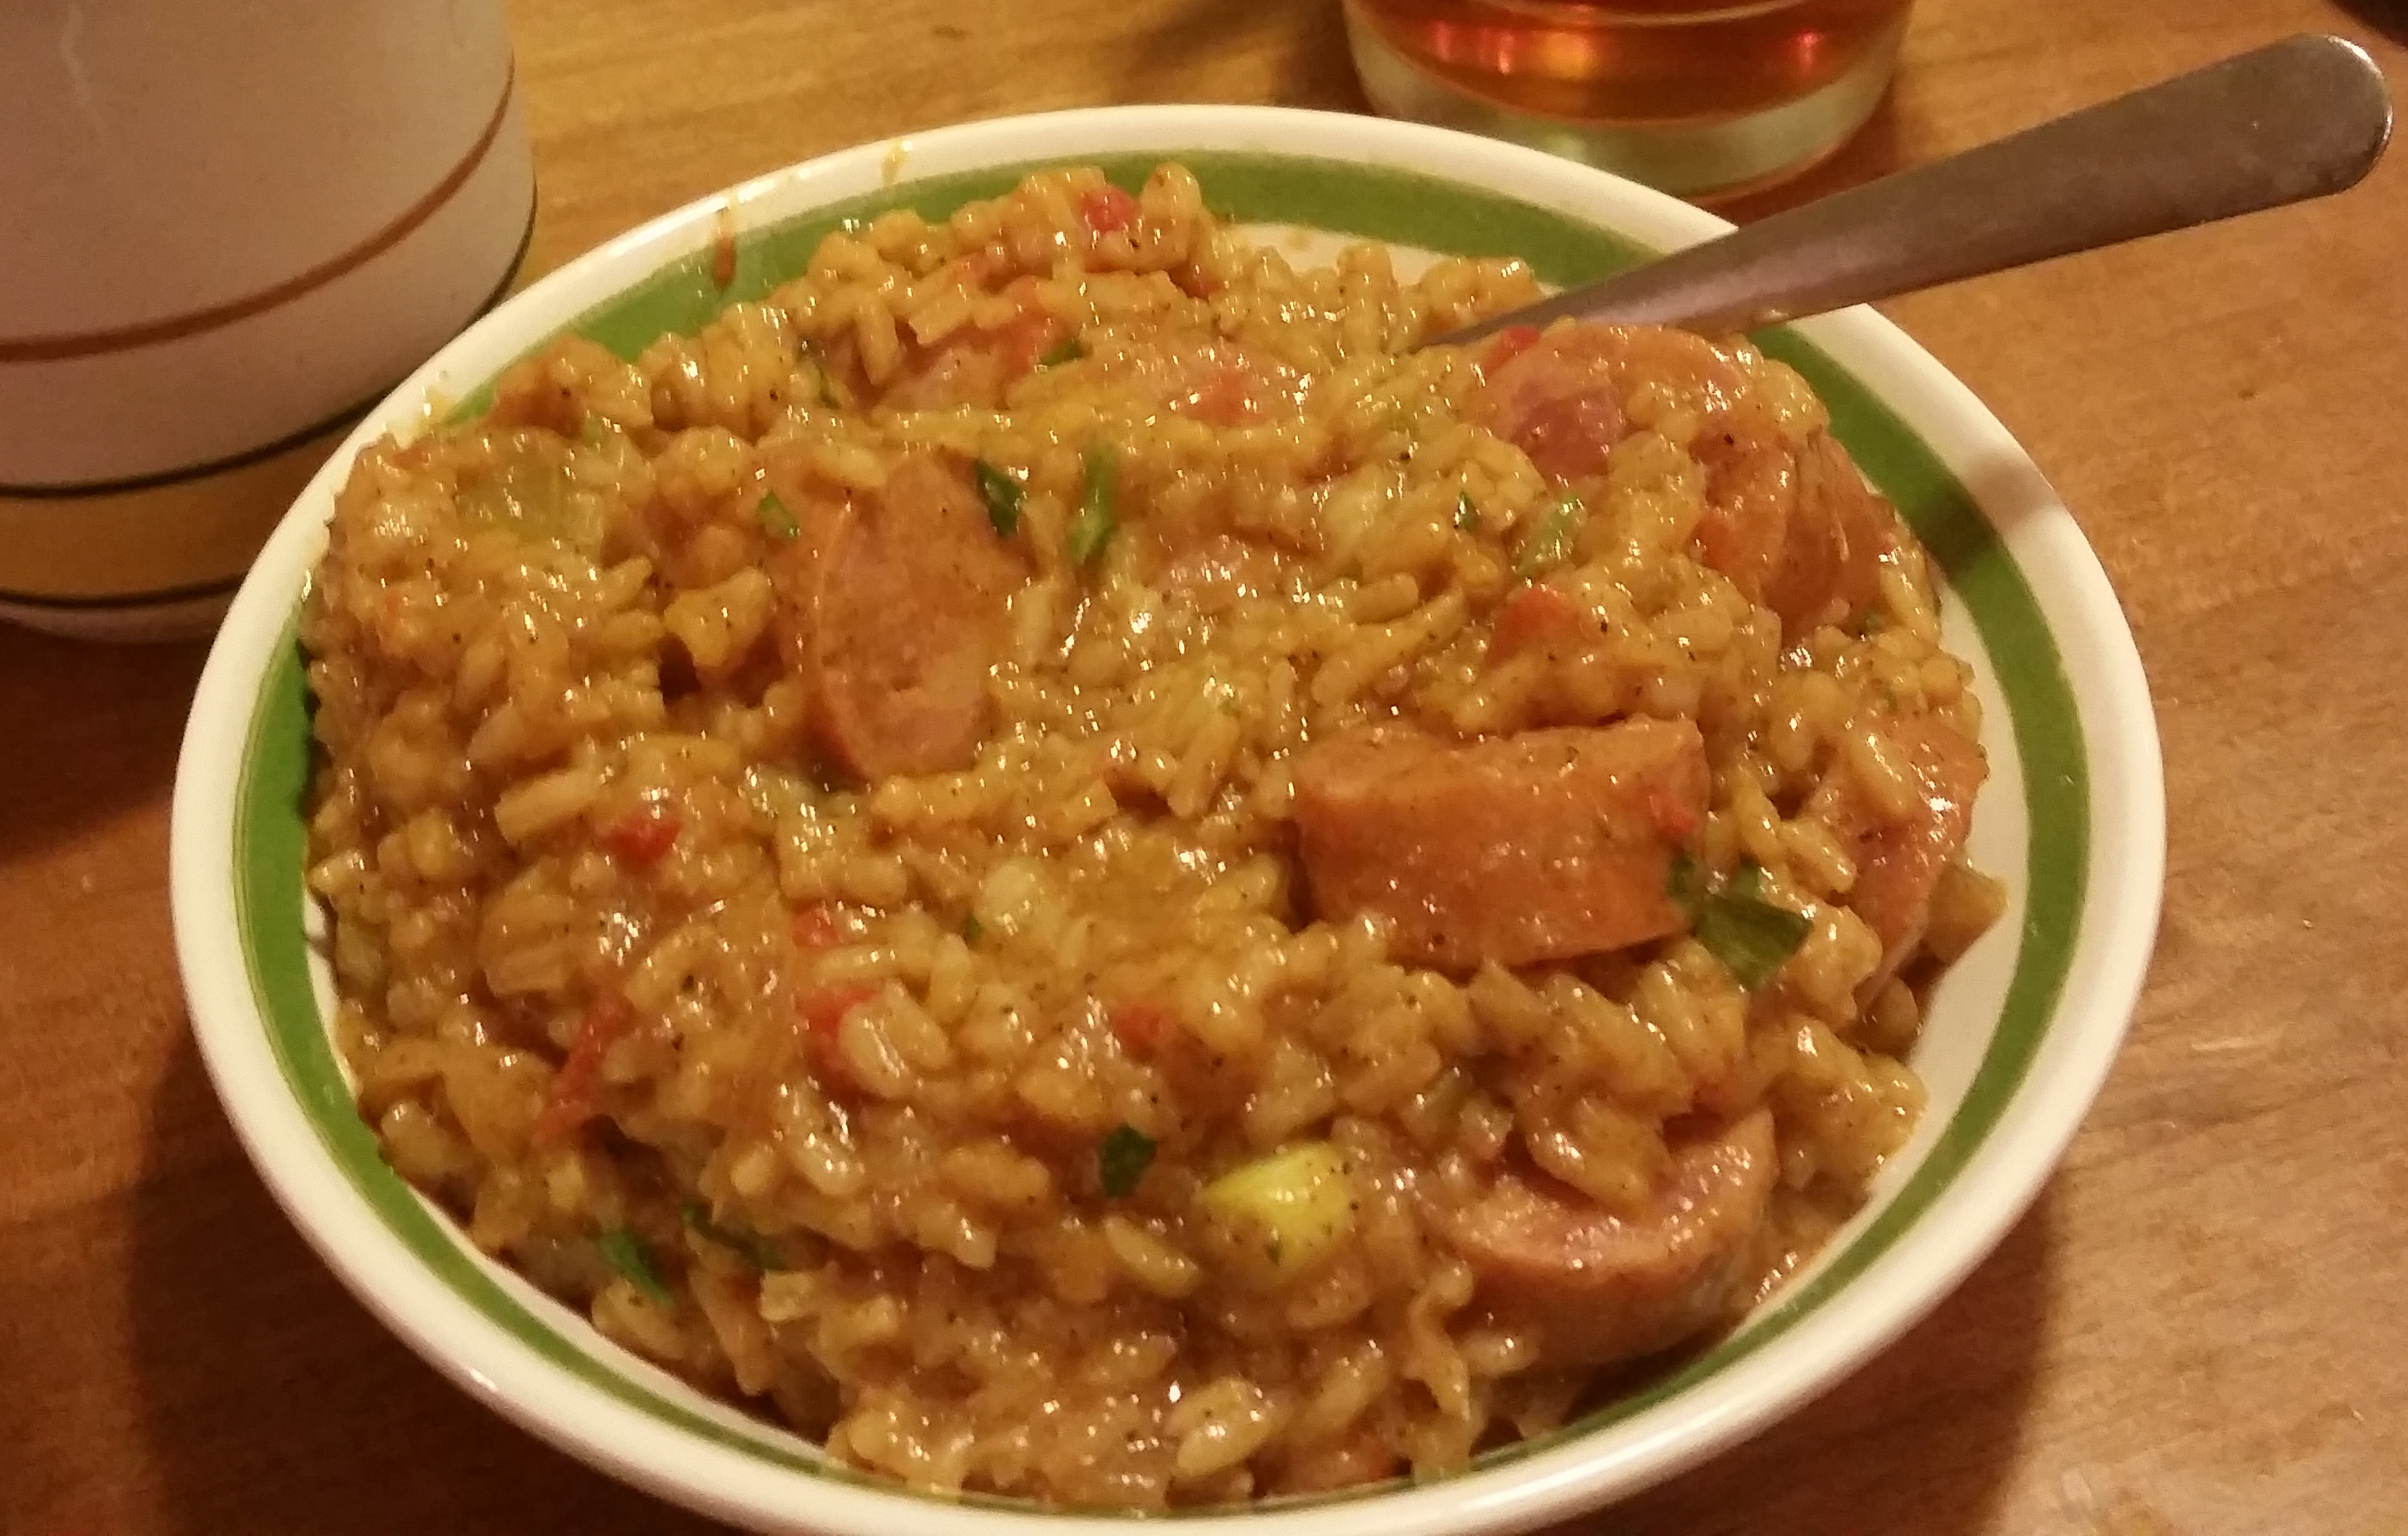
\includegraphics[height=\textheight]{cajun_jambalaya/finished.jpg}}
    \end{figure}

    \introduction{
    	This recipe again uses a mixture of spices, including that old standard Tony's Creole Seasoning along with various Paul Prudhomme spice mixes. Feel free to use other mixes you can get your hands on, or make you own spice mix. If you can find the Prudhomme spices and not the Tony’s, then at least buy the Redfish Magic which can substitute for all three if you don’t want to buy more than one mix.

    	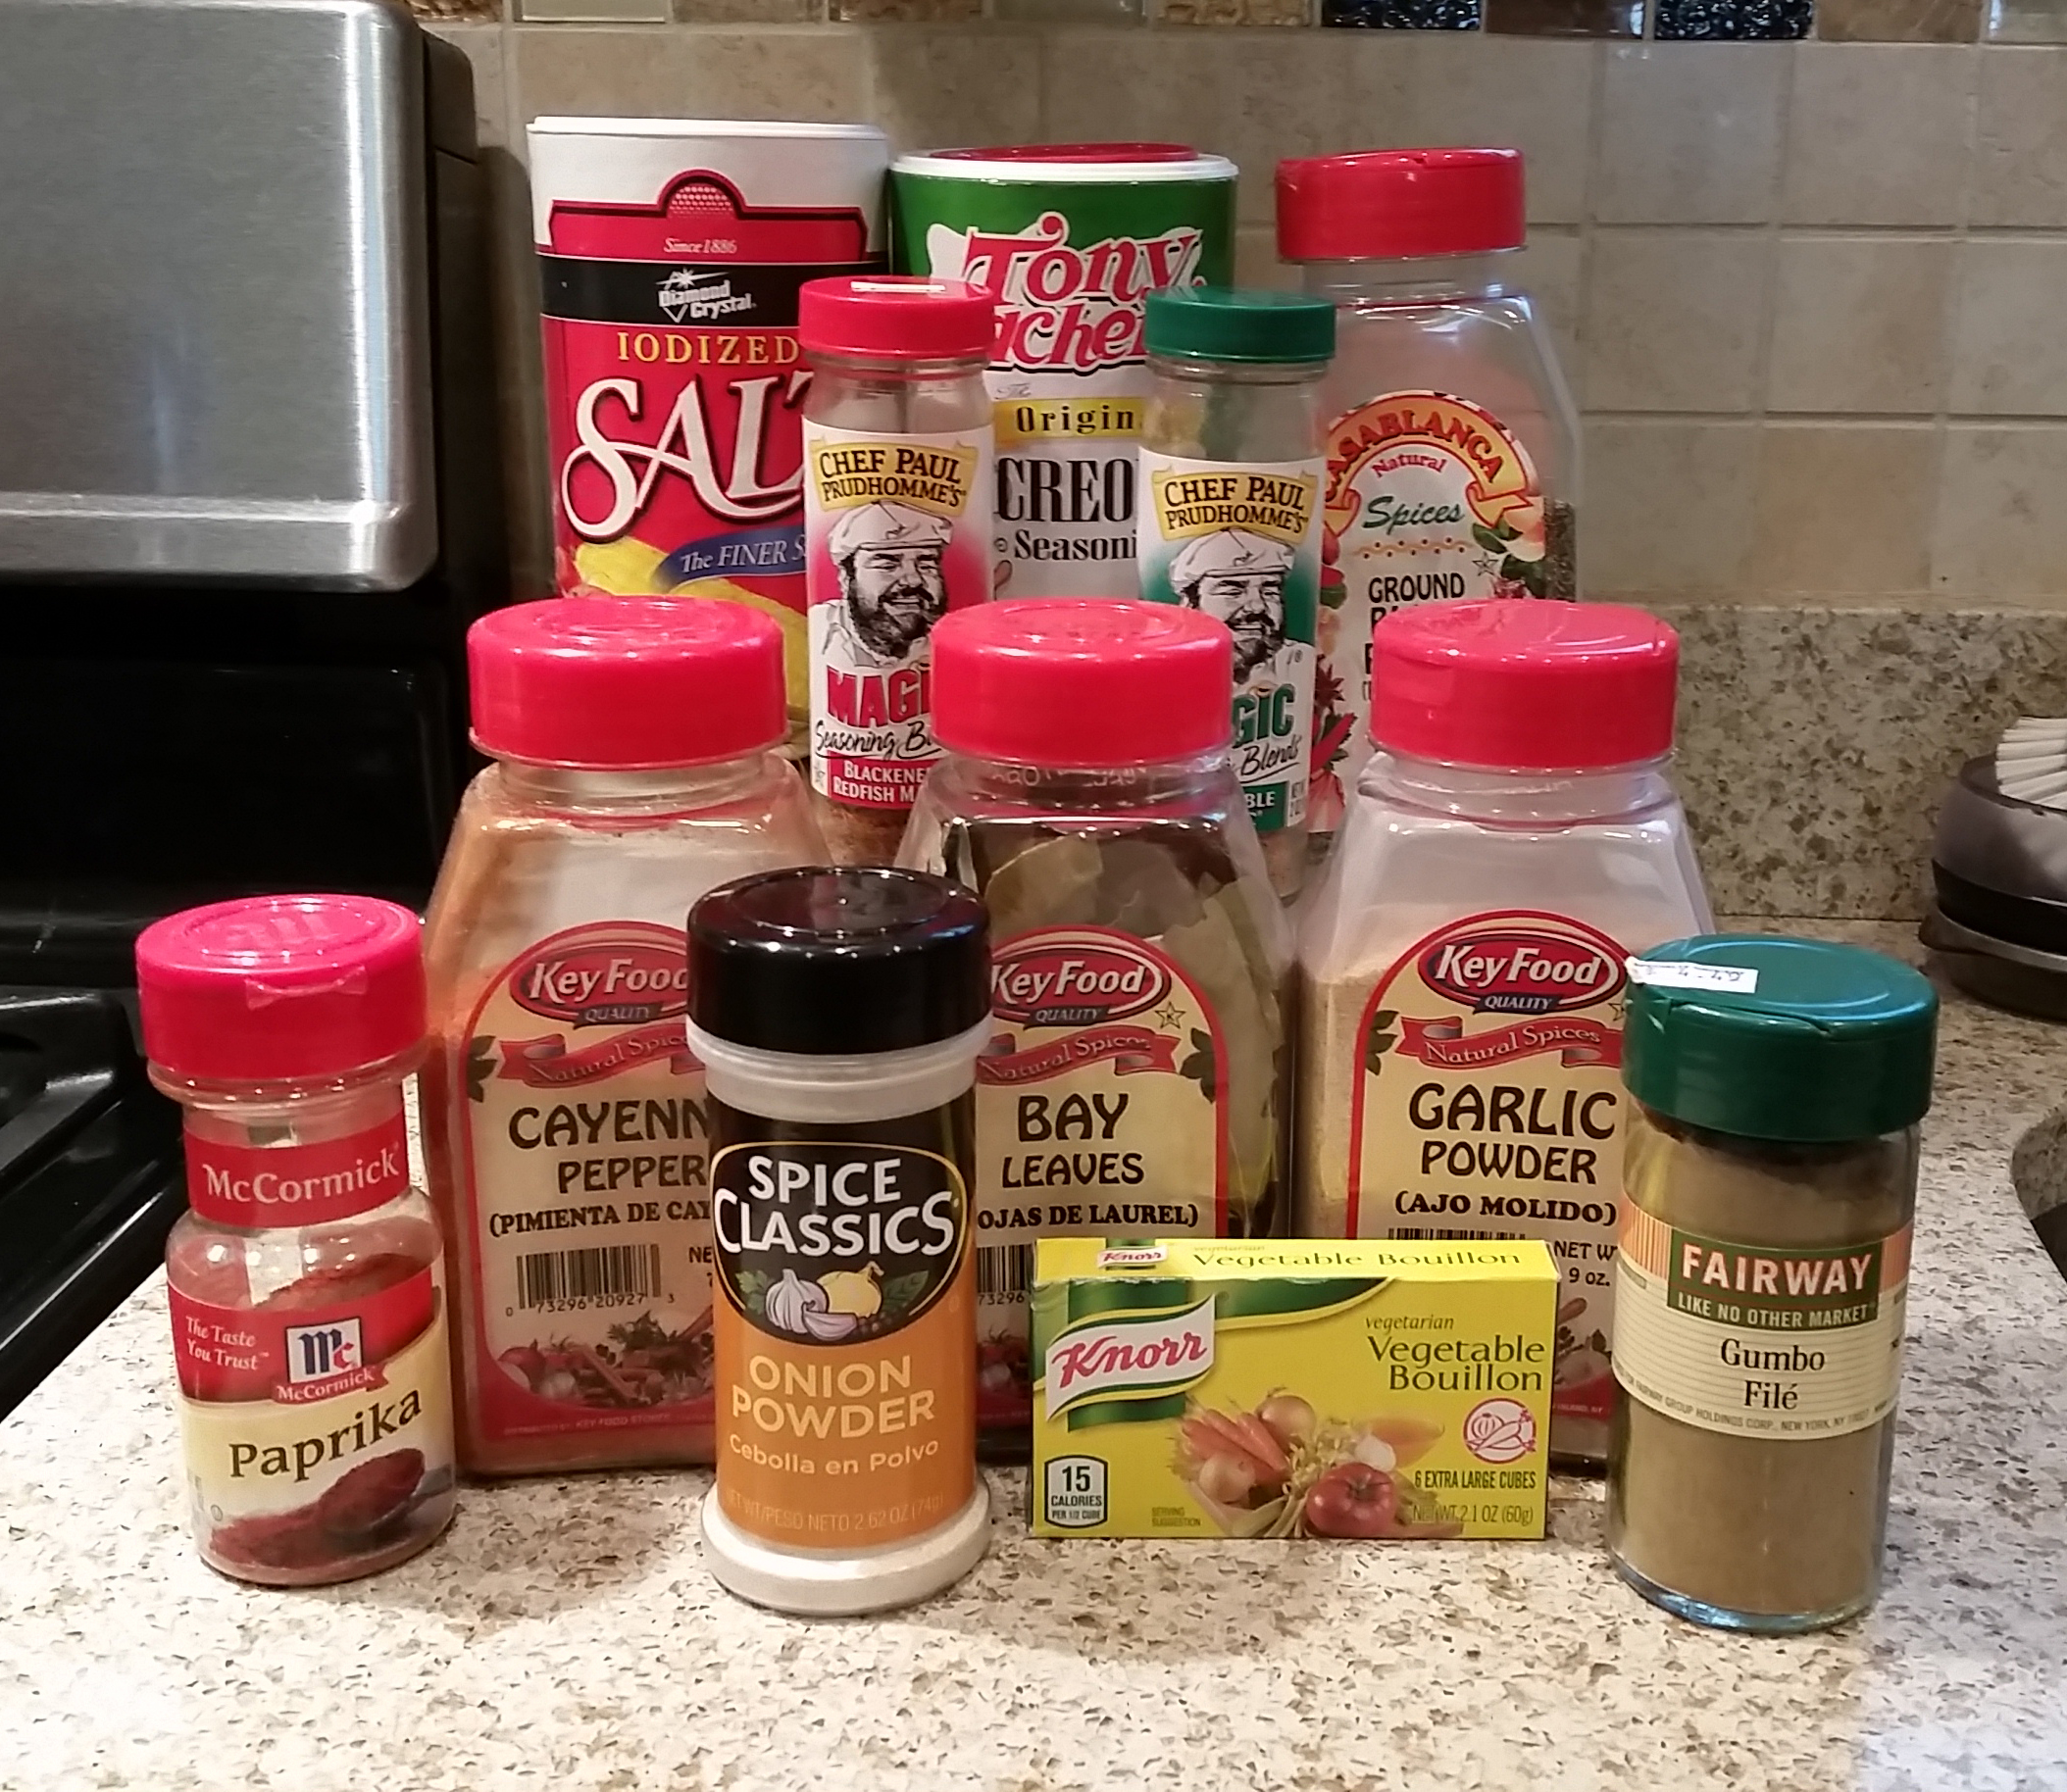
\includegraphics[width=\textwidth]{cajun_jambalaya/spices.jpg}

    	Also, this dish can be made vegan friendly by leaving the andouille out. You could also up the amount of vegetables to double what is called for here if you want it to make up for the lack of meat.
	}

	\ingredients[20]{
		\multicolumn{2}{c}{\textbf{Spices}} \\
		\SI{8}{\tablespoon} & Tony’s Creole Seasoning, split in half \\
		\SI{2x1/2}{\tablespoon} & Garlic powder \\
		\SI{2x1/2}{\tablespoon} & Onion powder \\
		\SI{2}{\tablespoon} & Cayenne pepper \\
		\SI{2}{\tablespoon} & Paul Prudhomme’s Vegetable Magic \\
		\SI{2}{\tablespoon} & Paul Prudhomme’s Redfish Magic \\
		\SI{1/2}{\tablespoon} & Paprika \\
		2--3 & Bay leaves \\
		& A small dash of Gumbo File (optional) \\
		1 & Vegetable bullion cube \\
		& Salt and pepper to taste (we used \SI{3/4}{\teaspoon} salt and \SI{1}{\tablespoon} of black pepper) \\
		\multicolumn{2}{c}{\textbf{All the rest}} \\
		\SI{5}{medium} & Bell peppers \\
		\SI{5}{stalks} & Celery \\
		\SI{1x1/2}{medium} & Onions \\
		\SI{1x1/4}{\cup} & Neutral oil, preferably canola, plus more to coat vegetables and bottom of pot \\
		\SI{6}{cups} & Rice \\
		\SI{8}{cups} & Vegetable broth \\
		\SI{4}{cups} & Water \\
		\SI{3}{\pound} & Andouille, sliced into bite sized rounds \\
		\SI{1/4}{\cup} & Thinly sliced scallions \\
		\SI{1/4}{\cup} & Roughly chopped parsley
	}

	\preparation{

		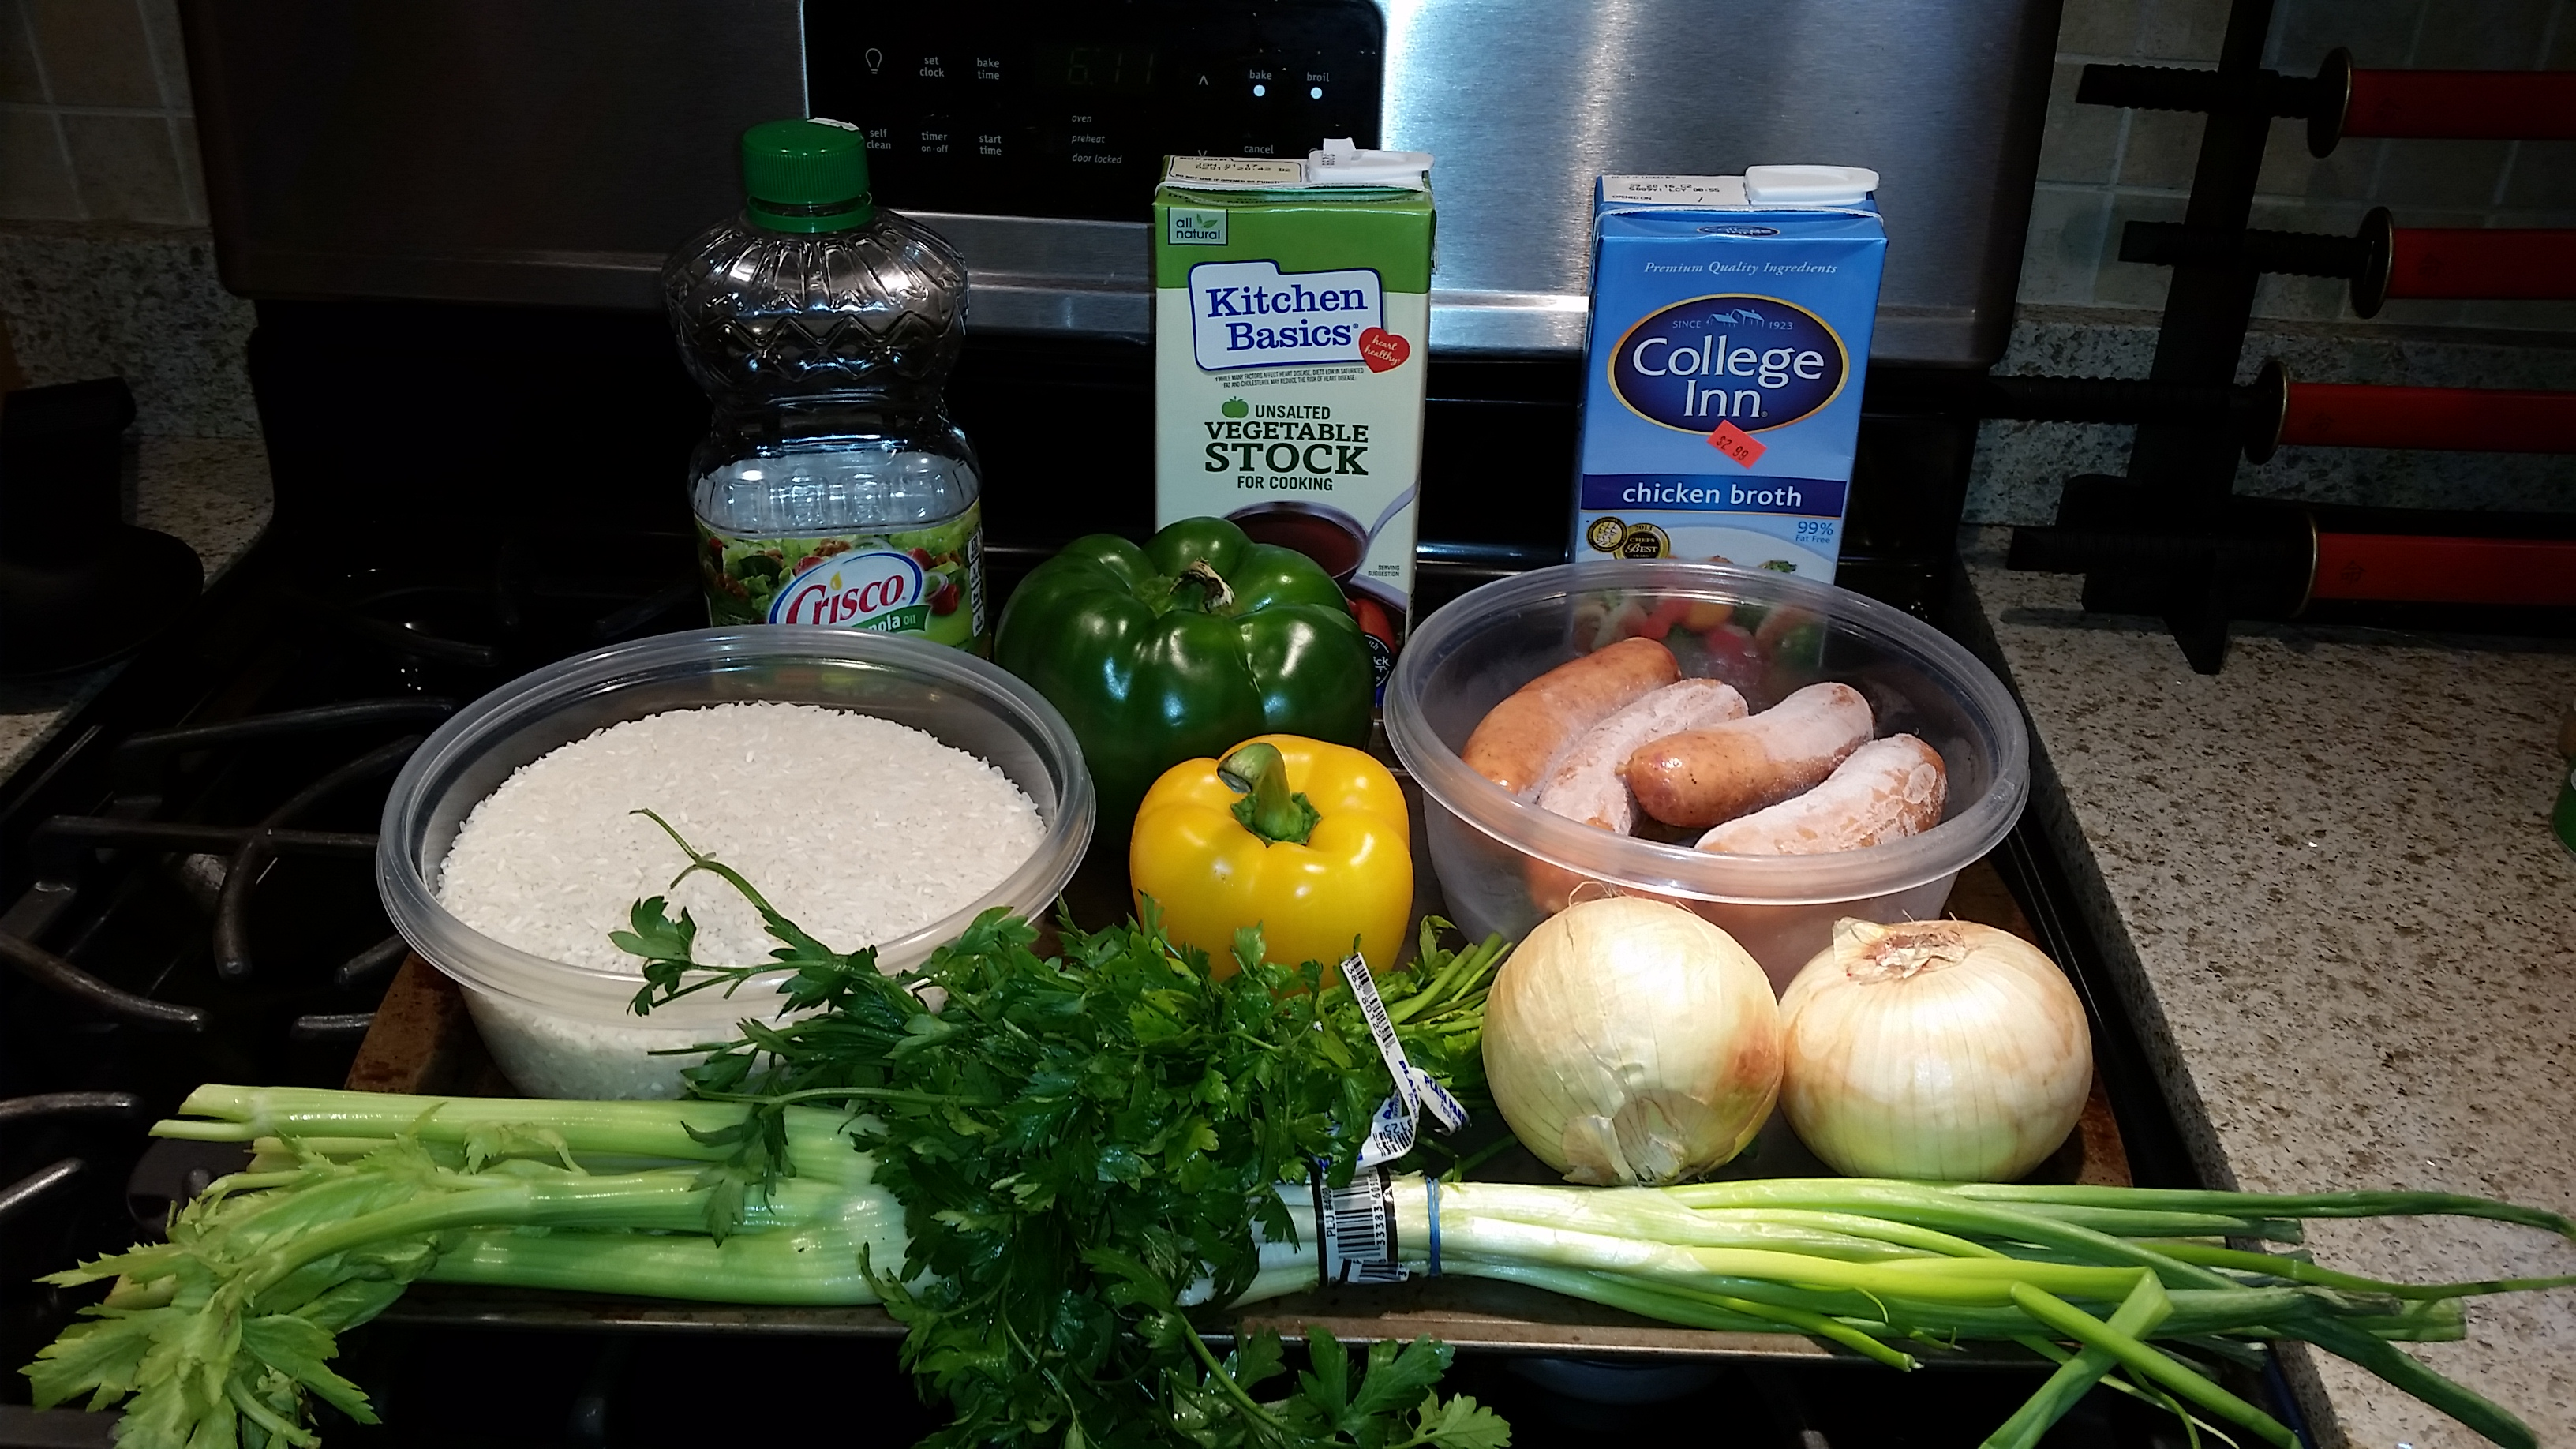
\includegraphics[width=0.52\textwidth]{cajun_jambalaya/20150829_181139.jpg}

		\step Chop the onions, pepper and celery into half inch pieces and throw them all in a bowl together. Pour enough oil over them to coat them and leave a small pool at the bottom of your bowl. Season with \SI{2}{\tablespoon} of Vegetable Magic. Let sit for about \SI{30}{\minute}.

		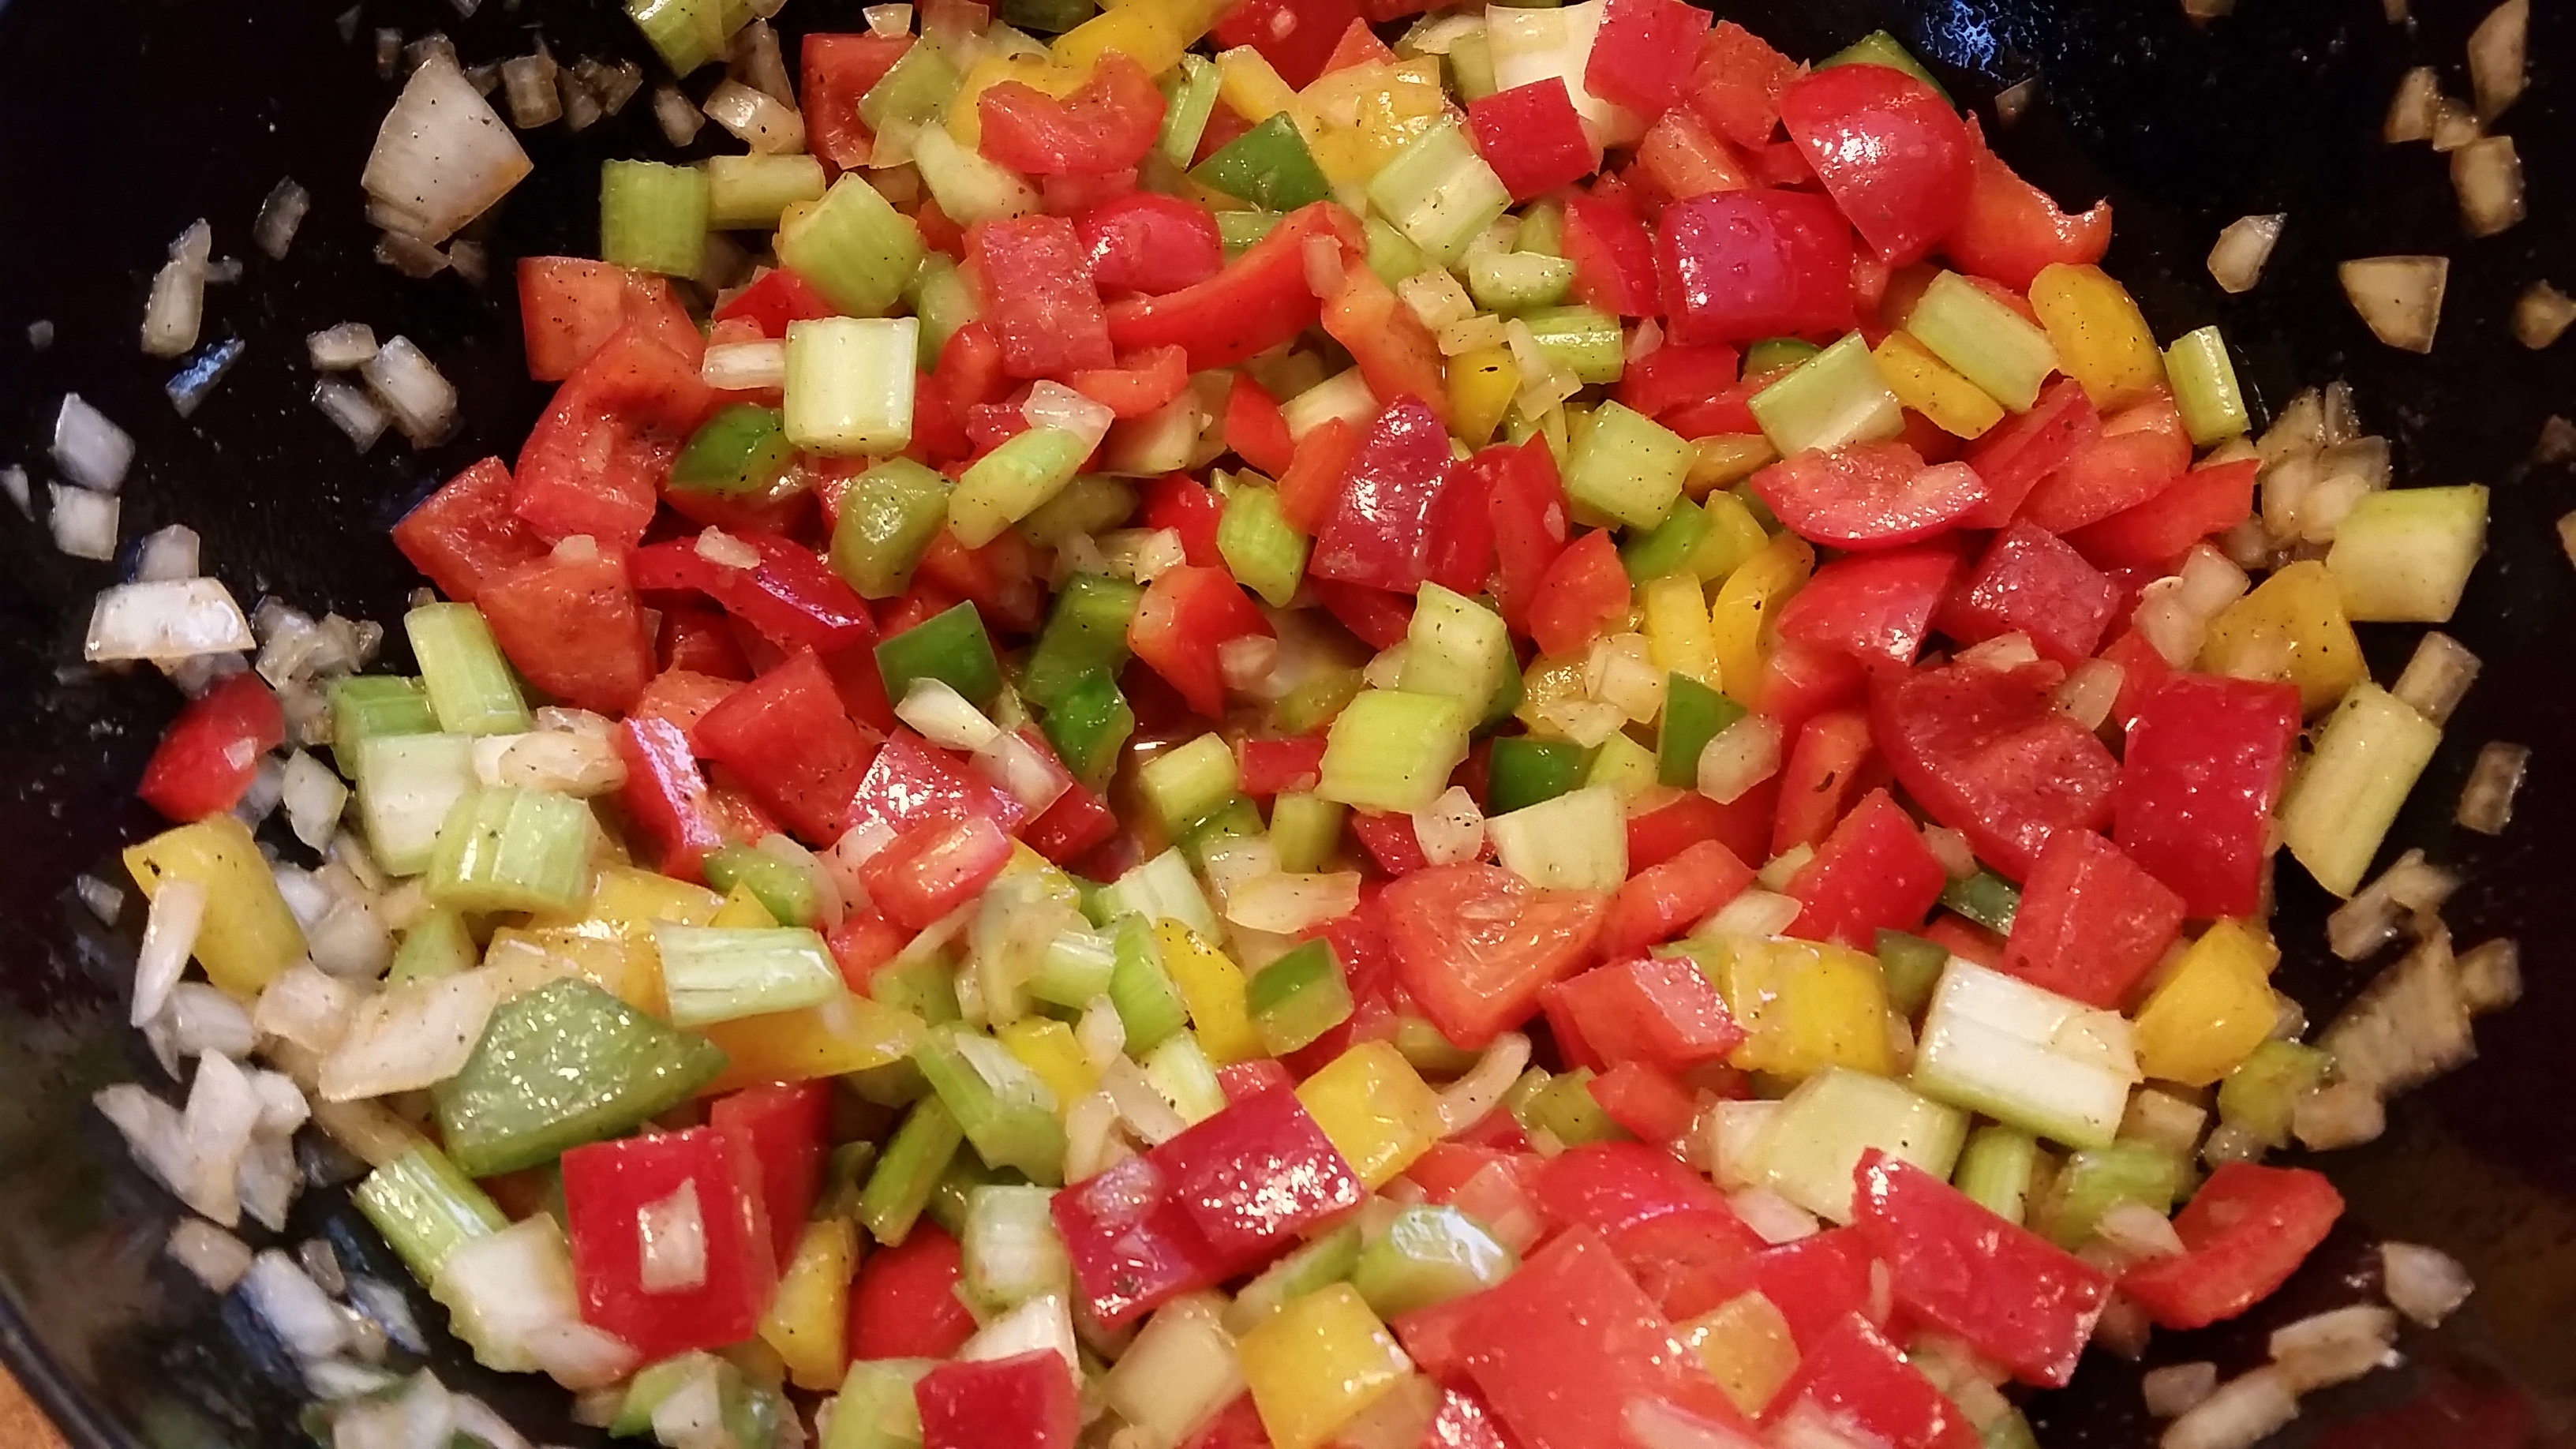
\includegraphics[width=0.52\textwidth]{cajun_jambalaya/20150829_181324.jpg}

		\step Place a pot that can hold at least 2\,gallons of liquid on a medium heat. Pour the vegetables and all the oil that comes with them. If the oil from the vegetables doesn't fully grease the bottom of your pot, add more until it does. Saute the vegetables until they are soft and translucent.

		\step Add in the water, vegetable stock, vegetable bullion cube, \SI{1x1/4}{\cup} of oil, bay leaves, and all of the other spices. Remember to add in some salt and pepper at this point, but don't go too heavy on the salt as most of the spice mixes have salt in them already.

		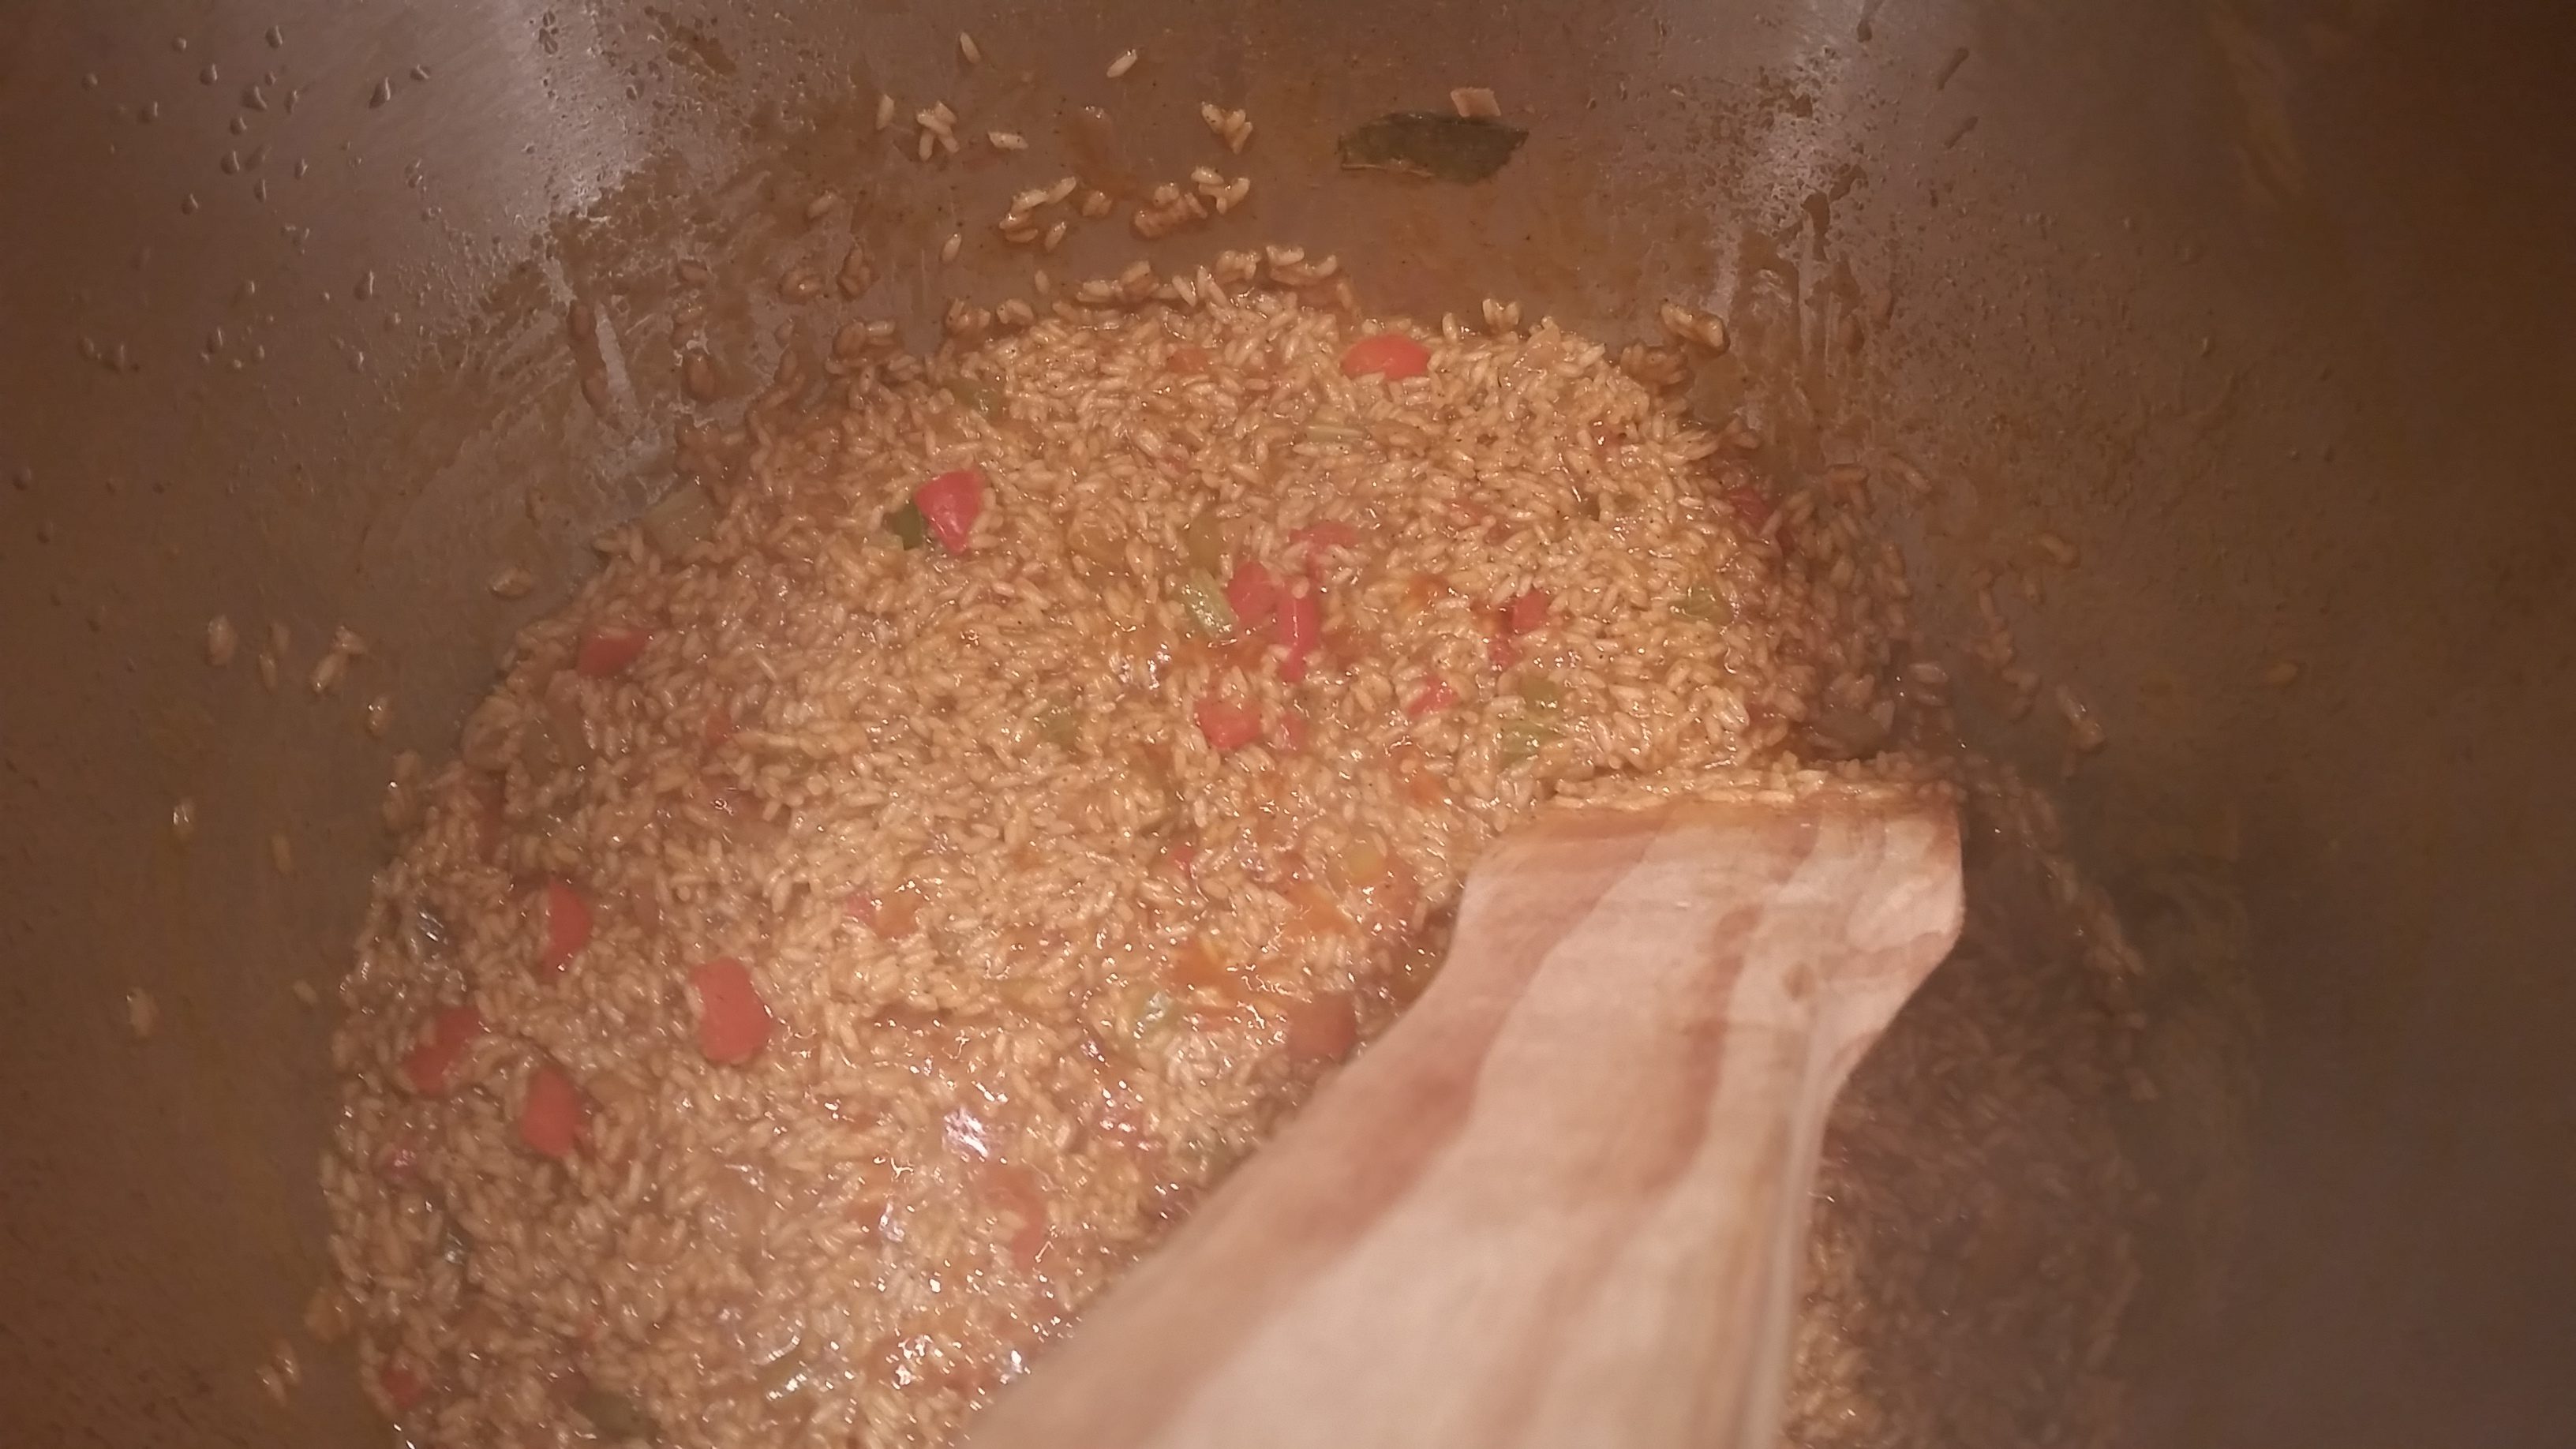
\includegraphics[width=\textwidth]{cajun_jambalaya/20150829_195533.jpg}

		\step Once the water is boiling, stir in the rice slowly. Make sure that the vegetables get evenly mixed throughout the rice and then reduce the heat to medium low. Stir very occasionally, making sure not to scrape the bottom of the pot. Rice may stick to the bottom and possibly burn, but don’t worry. That is usual and adds to the taste of the jambalaya.

		\step Cook until the water has been absorbed and the rice is soft. If the water evaporates before the rice is soft enough, feel free to add more water. Finding the right balance of heat and water for this process is finicky and will depend on the proportions you are making.

		\step Once the rice is cooked, add in the andouille, scallions and parsley and mix, again being careful not to scrape the over cooked rice off of the bottom of the pan. Season with further salt and pepper if needed.

		\step Serve hot and store the inevitable left overs in air tight containers in the freezer or fridge.

	}

\end{recipe}